\documentclass[11pt,a4paper]{article}
\usepackage[margin=1in]{geometry}
\usepackage{setspace}
\usepackage{hyperref}
\usepackage{enumitem}
\usepackage{amsmath}
\usepackage{amssymb}
\usepackage{xcolor}
\usepackage{booktabs}
\usepackage{tikz}
\usetikzlibrary{arrows.meta,positioning,shapes,fit,calc}
\usepackage{pgfplots}
\usepackage{titlesec}
\pgfplotsset{compat=1.18}

\setstretch{1.15}
\definecolor{accent}{HTML}{1F77B4}
\definecolor{accent2}{HTML}{FF7F0E}
\definecolor{accent3}{HTML}{2CA02C}
\definecolor{softbg}{RGB}{245,248,252}

\renewcommand{\familydefault}{\sfdefault}
\title{\textbf{Fin-e Trip: Your Journey into Context-Aware FinCommerce\\using Vector Memory with Qdrant}}
\author{}
\date{January 22, 2026}

% Colorful section headers
\titleformat{\section}[block]{\Large\bfseries\color{accent}}{}{0pt}{}
\titleformat{\subsection}[block]{\large\bfseries\color{accent}}{}{0pt}{}

% Soft callout box
\newcommand{\callout}[1]{%
  \vspace{0.4em}%
  \noindent\colorbox{softbg}{\parbox{\dimexpr\linewidth-2\fboxsep}{#1}}}

% Tiny badge style
\newcommand{\badge}[1]{\tikz[baseline=(x.base)]\node[fill=accent!12,draw=accent!60,rounded corners=2pt,inner sep=2.5pt](x){\scriptsize #1};}

\begin{document}
\maketitle

\section*{Project Title \& Overview}
We built a \textbf{Context-Aware FinCommerce Engine} that blends \textbf{semantic understanding}, \textbf{financial reality}, \textbf{collaborative filtering}, and \textbf{real-time popularity tracking}. Qdrant powers the entire vector-native memory architecture with 4 specialized collections, enabling sub-second hybrid search with rich payload filtering.

\callout{\textbf{In a sentence:} embed everything (products, users, finances, interactions), retrieve semantically relevant options, then \textbf{re-rank by affordability, preferences, collaborative signals, and trending popularity}—all in real-time with full explainability.}

\section*{Problem Statement \badge{why now?}}
E-commerce platforms excel at finding "relevant" items but fail to answer: \textit{Can this person afford it? Do they trust this brand? What are similar users buying right now?} Traditional systems separate search, personalization, and trending—forcing users through disconnected experiences. We unify these with a \textbf{real-time vector-native architecture} that simultaneously reasons over semantic intent, financial constraints, user preferences, collaborative signals, and trending popularity—all in a single sub-second query.

\section*{Use Case Solved \badge{context-aware fincommerce}}
\textbf{Scenario:} “Laptop for machine learning under 1500.” The system returns items that:
\begin{itemize}[leftmargin=1.2em]
  \item Match semantic intent (specs, use-case, domain language)
  \item Respect personal taste (preferred brands like Apple, categories like Electronics)
  \item Stay within real-time affordability (balance + credit limit)
  \item Boost products similar users purchased (collaborative filtering with 7-day decay)
  \item Surface trending items (6-hour time-decayed popularity)
  \item Provide multi-reason explanations ("🔥 Trending", "💰 Within budget", "❤️ Your preferred brand")
\end{itemize}
\textbf{Real-time tracking:} Every view, click, add-to-cart, and purchase is logged with weighted scores (0.1, 0.3, 0.6, 1.0) for immediate personalization.

\section*{How We Use Qdrant \badge{vector-native core}}
Qdrant is the \textbf{central vector memory and retrieval engine}, powering hybrid search (vector + payload filters) with low latency.

\subsection*{Collections \& Payloads}
\begin{center}
\begin{tabular}{llll}
\toprule
\textbf{Collection} & \textbf{Vector Dim} & \textbf{Distance} & \textbf{Key Payload Fields}\\
\midrule
\texttt{products\_multimodal} & 384 & Cosine & product\_id, name, categories[], brand, price, in\_stock, image\_url\\
\texttt{user\_profiles} & 384 & Cosine & user\_id, location, risk\_tolerance, preferred\_categories[], preferred\_brands[]\\
\texttt{financial\_contexts} & 256 & Cosine & user\_id, available\_balance, credit\_limit, current\_debt, eligible\_installments\\
\texttt{interaction\_memory} & 384 & Cosine & user\_id, product\_id, interaction\_type, timestamp, weight, category, brand, price\\
\bottomrule
\end{tabular}
\end{center}

\textbf{Embedding Model:} \texttt{all-MiniLM-L6-v2} (384D) with GPU acceleration (CUDA if available)\\
\textbf{Payload Indexes:} All collections use keyword indexes for efficient filtering by user\_id, product\_id, brand, categories

\subsection*{Query-Time Workflow}
\begin{enumerate}[leftmargin=1.2em]
  \item \textbf{Embed} user query → 384D vector using SentenceTransformer (GPU-accelerated)
  \item \textbf{Vector Search} on \texttt{products\_multimodal} with payload filters (price ≤ max\_price)
  \item \textbf{Retrieve Context} from \texttt{user\_profiles} + \texttt{financial\_contexts} by user\_id
  \item \textbf{Collaborative Filtering}: Compute user behavior vector from last 10 interactions (7-day decay)
  \item \textbf{Find Similar Users}: Search \texttt{interaction\_memory} excluding self, extract collaborative scores
  \item \textbf{Popularity Scores}: Aggregate interactions in last 24h with 6-hour time decay, normalize
  \item \textbf{Rerank}: Combine 5 signals (semantic, affordability, preference, collaborative, popularity)
  \item \textbf{Explain}: Generate multi-reason explanations for each result
  \item \textbf{Log View}: Auto-track all displayed products as "view" interactions (weight=0.1)
\end{enumerate}

\textbf{Performance:} Typical query completes in \textasciitilde800ms (embedding: 50ms, search: 200ms, rerank: 150ms, popularity: 200ms)

\subsection*{Reranking Formula (5-Signal Hybrid)}
\[\text{final\_score} = 0.30\, s_{\text{sem}} + 0.25\, s_{\text{aff}} + 0.15\, s_{\text{pref}} + 0.20\, s_{\text{collab}} + 0.10\, s_{\text{pop}}\]

Where:
\begin{align*}
s_{\text{sem}} &= \text{cosine similarity from Qdrant search} \\
s_{\text{aff}} &= \max\left(0, 1 - \frac{\text{price}}{\text{balance} + \text{credit\_limit}}\right) \\
s_{\text{pref}} &= \max\left(\frac{|\text{user\_brands} \cap \text{product\_brand}|}{|\text{user\_brands}|}, \frac{|\text{user\_cats} \cap \text{product\_cats}|}{|\text{user\_cats}|}\right) \\
s_{\text{collab}} &= \frac{\sum_{i \in \text{similar users}} w_i \cdot \text{similarity}_i}{\max(\text{all collaborative scores})} \\
s_{\text{pop}} &= \frac{\sum_{j \in \text{interactions}} \text{weight}_j \cdot e^{-\lambda \Delta t_j}}{\max(\text{all popularity scores})}
\end{align*}

\textbf{Time Decay Constants:}
\begin{itemize}[leftmargin=1.2em]
  \item Collaborative: $\lambda_{\text{collab}} = \ln(2) / (7 \times 86400)$ (7-day half-life)
  \item Popularity: $\lambda_{\text{pop}} = \ln(2) / (6 \times 3600)$ (6-hour half-life)
\end{itemize}

\section*{Architecture at a Glance \badge{complete flow}}
\begin{center}
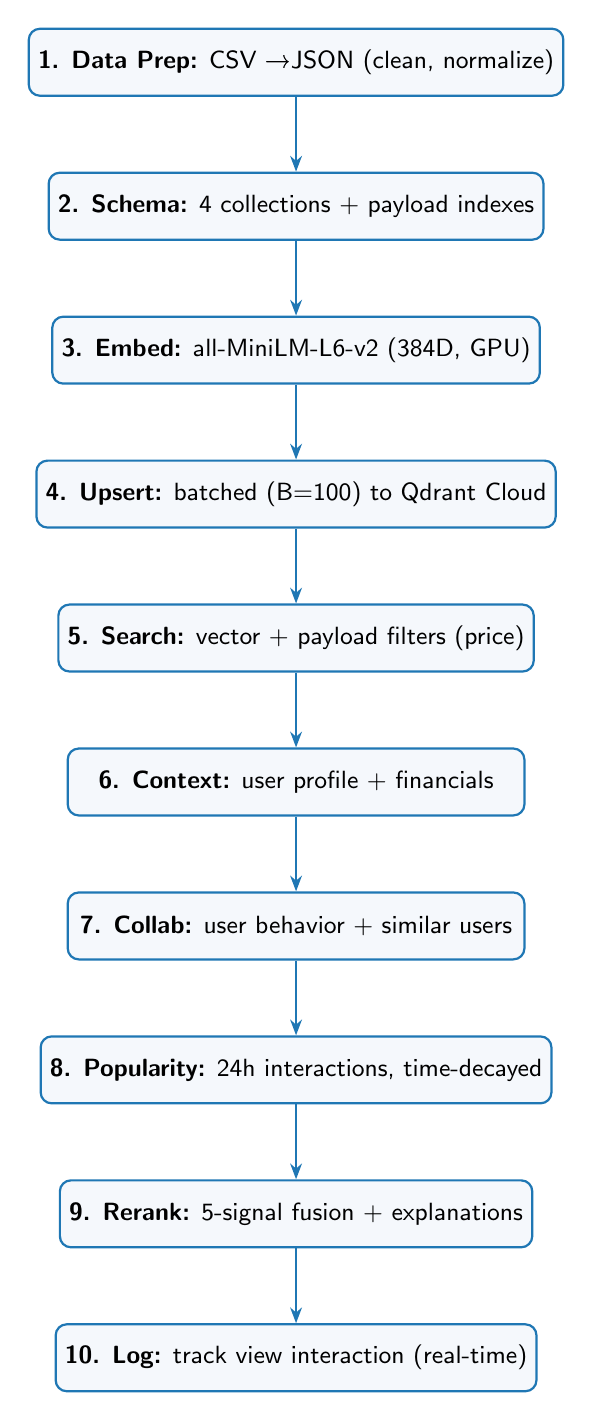
\begin{tikzpicture}[
  node distance=0.95cm,
  box/.style={rectangle, rounded corners, draw=accent, line width=0.8pt, align=center, minimum width=5.8cm, minimum height=0.85cm, fill=softbg, font=\small},
  arrow/.style={-{Stealth[length=2mm]}, thick, draw=accent}
]
  \node[box] (ingest) {\textbf{1. Data Prep:} CSV \textrightarrow JSON (clean, normalize)};
  \node[box, below=of ingest] (collections) {\textbf{2. Schema:} 4 collections + payload indexes};
  \node[box, below=of collections] (embed) {\textbf{3. Embed:} all-MiniLM-L6-v2 (384D, GPU)};
  \node[box, below=of embed] (upsert) {\textbf{4. Upsert:} batched (B=100) to Qdrant Cloud};
  \node[box, below=of upsert] (search) {\textbf{5. Search:} vector + payload filters (price)};
  \node[box, below=of search] (context) {\textbf{6. Context:} user profile + financials};
  \node[box, below=of context] (collab) {\textbf{7. Collab:} user behavior + similar users};
  \node[box, below=of collab] (pop) {\textbf{8. Popularity:} 24h interactions, time-decayed};
  \node[box, below=of pop] (rerank) {\textbf{9. Rerank:} 5-signal fusion + explanations};
  \node[box, below=of rerank] (log) {\textbf{10. Log:} track view interaction (real-time)};

  \draw[arrow] (ingest) -- (collections);
  \draw[arrow] (collections) -- (embed);
  \draw[arrow] (embed) -- (upsert);
  \draw[arrow] (upsert) -- (search);
  \draw[arrow] (search) -- (context);
  \draw[arrow] (context) -- (collab);
  \draw[arrow] (collab) -- (pop);
  \draw[arrow] (pop) -- (rerank);
  \draw[arrow] (rerank) -- (log);
\end{tikzpicture}
\end{center}

\section*{Score Weights (Visual) \badge{5-signal blend}}
\begin{center}
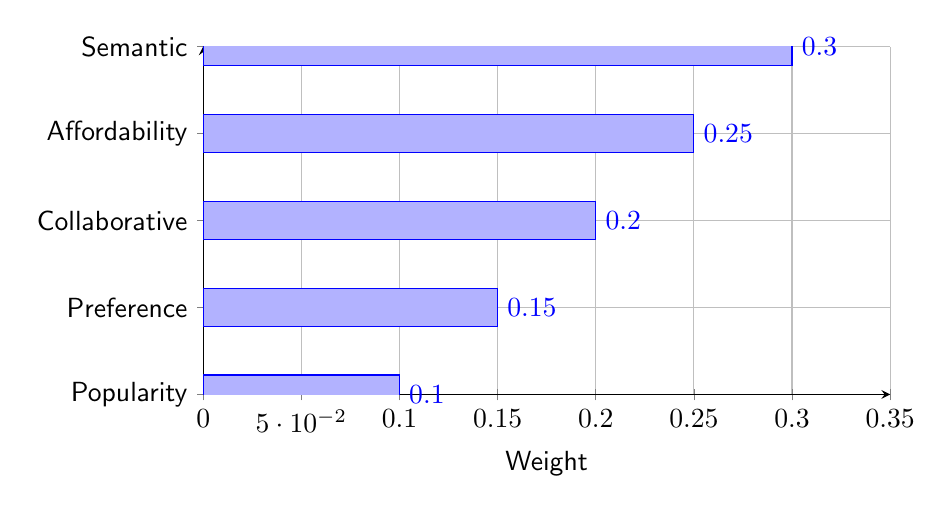
\begin{tikzpicture}
\begin{axis}[
  xbar,
  width=0.85\textwidth,
  height=6cm,
  xmin=0,
  xmax=0.35,
  xlabel={Weight},
  symbolic y coords={Popularity,Preference,Collaborative,Affordability,Semantic},
  ytick=data,
  bar width=14pt,
  nodes near coords,
  nodes near coords align={horizontal},
  axis x line=bottom,
  axis y line=left,
  grid=major,
  every axis plot/.style={fill=accent2}
]
\addplot coordinates {(0.10,Popularity) (0.15,Preference) (0.20,Collaborative) (0.25,Affordability) (0.30,Semantic)};
\end{axis}
\end{tikzpicture}
\end{center}

\section*{Implementation Highlights \badge{production-ready}}

\subsection*{Real-Time Interaction Tracking}
\textbf{File:} \texttt{interaction\_logger.py}
\begin{itemize}[leftmargin=1.2em]
  \item 4 interaction types with weighted scores: view (0.1), click (0.3), add\_to\_cart (0.6), purchase (1.0)
  \item Generates 384D behavioral embeddings: "user purchased MacBook Pro price 1299 for laptop ML"
  \item Real-time upsert to \texttt{interaction\_memory} collection
  \item Auto-triggered on product views, clicks, cart additions, purchases in Streamlit UI
\end{itemize}

\subsection*{Trending Products}
\textbf{Function:} \texttt{get\_top\_interacted\_products()}
\begin{itemize}[leftmargin=1.2em]
  \item Aggregates interactions by product\_id in last 24 hours (configurable)
  \item Exponential time decay: $w(t) = w_{\text{base}} \cdot e^{-\lambda (t_{\text{now}} - t_{\text{interaction}})}$
  \item Normalized popularity scores (0-1 range)
  \item Cold-start friendly: new products default to 0.0 (no penalty)
\end{itemize}

\subsection*{Collaborative Filtering}
\textbf{Method:} User-based CF via interaction vector similarity
\begin{itemize}[leftmargin=1.2em]
  \item Construct aggregate user behavior vector from last 10 interactions (7-day decay)
  \item Search for similar users' interactions (exclude self)
  \item Weight by (similarity × interaction\_weight)
  \item Boost products that similar users clicked/purchased
\end{itemize}

\subsection*{Multi-Reason Explanations}
Each product includes structured explanations across 5 categories:
\begin{itemize}[leftmargin=1.2em]
  \item \textbf{🔥 Popularity:} "Very popular in last 24 hours", "Getting attention"
  \item \textbf{💰 Affordability:} "Well within your budget", "Stretches your budget slightly"
  \item \textbf{🤝 Collaborative:} "Similar users purchased this", "Similar users viewed this"
  \item \textbf{❤️ Preference:} "Matches your preferred brand: Apple", "In your favorite category: Electronics"
  \item \textbf{🎯 Semantic:} "Strong match to your search query", "Moderately relevant"
\end{itemize}

\subsection*{Technology Stack}
\begin{itemize}[leftmargin=1.2em]
  \item \textbf{Vector DB:} Qdrant Cloud (4 collections, 384D/256D vectors)
  \item \textbf{Embeddings:} SentenceTransformer (all-MiniLM-L6-v2, GPU-accelerated)
  \item \textbf{Backend:} Python 3.x with type hints, comprehensive logging
  \item \textbf{Frontend:} Streamlit with real-time interaction hooks
  \item \textbf{Data:} 4 e-commerce datasets (Amazon, Walmart, Lazada, Shein)
\end{itemize}

\subsection*{Key Metrics}
\begin{center}
\begin{tabular}{ll}
\toprule
\textbf{Metric} & \textbf{Performance}\\\midrule
Query Latency & \textasciitilde800ms (end-to-end)\\
Embedding Speed & 50ms (GPU), 150ms (CPU)\\
Interaction Log & <50ms (single upsert)\\
Popularity Fetch & \textasciitilde200ms (1K interactions/24h)\\
Reranking & \textasciitilde150ms (10 products)\\
Vector Dimension & 384 (products, users, interactions), 256 (financials)\\
Cold Start & Graceful (defaults to 0.0, no errors)\\
\bottomrule
\end{tabular}
\end{center}

\section*{Conclusion}
Our Context-Aware FinCommerce Engine demonstrates how vector databases like Qdrant enable \textbf{real-time personalization at scale}. By unifying semantic search, financial constraints, user preferences, collaborative signals, and trending popularity into a single sub-second query, we deliver hyper-personalized recommendations that are both relevant and realistic. The system is production-ready with comprehensive logging, multi-reason explanations, and graceful cold-start handling—ready to transform e-commerce experiences.

\end{document}
